\documentclass{article} % For LaTeX2e
\usepackage{iclr2026_conference,times}

% Optional math commands from https://github.com/goodfeli/dlbook_notation.
%%%%% NEW MATH DEFINITIONS %%%%%

\usepackage{amsmath,amsfonts,bm}

% Mark sections of captions for referring to divisions of figures
\newcommand{\figleft}{{\em (Left)}}
\newcommand{\figcenter}{{\em (Center)}}
\newcommand{\figright}{{\em (Right)}}
\newcommand{\figtop}{{\em (Top)}}
\newcommand{\figbottom}{{\em (Bottom)}}
\newcommand{\captiona}{{\em (a)}}
\newcommand{\captionb}{{\em (b)}}
\newcommand{\captionc}{{\em (c)}}
\newcommand{\captiond}{{\em (d)}}

% Highlight a newly defined term
\newcommand{\newterm}[1]{{\bf #1}}


% Figure reference, lower-case.
\def\figref#1{figure~\ref{#1}}
% Figure reference, capital. For start of sentence
\def\Figref#1{Figure~\ref{#1}}
\def\twofigref#1#2{figures \ref{#1} and \ref{#2}}
\def\quadfigref#1#2#3#4{figures \ref{#1}, \ref{#2}, \ref{#3} and \ref{#4}}
% Section reference, lower-case.
\def\secref#1{section~\ref{#1}}
% Section reference, capital.
\def\Secref#1{Section~\ref{#1}}
% Reference to two sections.
\def\twosecrefs#1#2{sections \ref{#1} and \ref{#2}}
% Reference to three sections.
\def\secrefs#1#2#3{sections \ref{#1}, \ref{#2} and \ref{#3}}
% Reference to an equation, lower-case.
\def\eqref#1{equation~\ref{#1}}
% Reference to an equation, upper case
\def\Eqref#1{Equation~\ref{#1}}
% A raw reference to an equation---avoid using if possible
\def\plaineqref#1{\ref{#1}}
% Reference to a chapter, lower-case.
\def\chapref#1{chapter~\ref{#1}}
% Reference to an equation, upper case.
\def\Chapref#1{Chapter~\ref{#1}}
% Reference to a range of chapters
\def\rangechapref#1#2{chapters\ref{#1}--\ref{#2}}
% Reference to an algorithm, lower-case.
\def\algref#1{algorithm~\ref{#1}}
% Reference to an algorithm, upper case.
\def\Algref#1{Algorithm~\ref{#1}}
\def\twoalgref#1#2{algorithms \ref{#1} and \ref{#2}}
\def\Twoalgref#1#2{Algorithms \ref{#1} and \ref{#2}}
% Reference to a part, lower case
\def\partref#1{part~\ref{#1}}
% Reference to a part, upper case
\def\Partref#1{Part~\ref{#1}}
\def\twopartref#1#2{parts \ref{#1} and \ref{#2}}

\def\ceil#1{\lceil #1 \rceil}
\def\floor#1{\lfloor #1 \rfloor}
\def\1{\bm{1}}
\newcommand{\train}{\mathcal{D}}
\newcommand{\valid}{\mathcal{D_{\mathrm{valid}}}}
\newcommand{\test}{\mathcal{D_{\mathrm{test}}}}

\def\eps{{\epsilon}}


% Random variables
\def\reta{{\textnormal{$\eta$}}}
\def\ra{{\textnormal{a}}}
\def\rb{{\textnormal{b}}}
\def\rc{{\textnormal{c}}}
\def\rd{{\textnormal{d}}}
\def\re{{\textnormal{e}}}
\def\rf{{\textnormal{f}}}
\def\rg{{\textnormal{g}}}
\def\rh{{\textnormal{h}}}
\def\ri{{\textnormal{i}}}
\def\rj{{\textnormal{j}}}
\def\rk{{\textnormal{k}}}
\def\rl{{\textnormal{l}}}
% rm is already a command, just don't name any random variables m
\def\rn{{\textnormal{n}}}
\def\ro{{\textnormal{o}}}
\def\rp{{\textnormal{p}}}
\def\rq{{\textnormal{q}}}
\def\rr{{\textnormal{r}}}
\def\rs{{\textnormal{s}}}
\def\rt{{\textnormal{t}}}
\def\ru{{\textnormal{u}}}
\def\rv{{\textnormal{v}}}
\def\rw{{\textnormal{w}}}
\def\rx{{\textnormal{x}}}
\def\ry{{\textnormal{y}}}
\def\rz{{\textnormal{z}}}

% Random vectors
\def\rvepsilon{{\mathbf{\epsilon}}}
\def\rvtheta{{\mathbf{\theta}}}
\def\rva{{\mathbf{a}}}
\def\rvb{{\mathbf{b}}}
\def\rvc{{\mathbf{c}}}
\def\rvd{{\mathbf{d}}}
\def\rve{{\mathbf{e}}}
\def\rvf{{\mathbf{f}}}
\def\rvg{{\mathbf{g}}}
\def\rvh{{\mathbf{h}}}
\def\rvu{{\mathbf{i}}}
\def\rvj{{\mathbf{j}}}
\def\rvk{{\mathbf{k}}}
\def\rvl{{\mathbf{l}}}
\def\rvm{{\mathbf{m}}}
\def\rvn{{\mathbf{n}}}
\def\rvo{{\mathbf{o}}}
\def\rvp{{\mathbf{p}}}
\def\rvq{{\mathbf{q}}}
\def\rvr{{\mathbf{r}}}
\def\rvs{{\mathbf{s}}}
\def\rvt{{\mathbf{t}}}
\def\rvu{{\mathbf{u}}}
\def\rvv{{\mathbf{v}}}
\def\rvw{{\mathbf{w}}}
\def\rvx{{\mathbf{x}}}
\def\rvy{{\mathbf{y}}}
\def\rvz{{\mathbf{z}}}

% Elements of random vectors
\def\erva{{\textnormal{a}}}
\def\ervb{{\textnormal{b}}}
\def\ervc{{\textnormal{c}}}
\def\ervd{{\textnormal{d}}}
\def\erve{{\textnormal{e}}}
\def\ervf{{\textnormal{f}}}
\def\ervg{{\textnormal{g}}}
\def\ervh{{\textnormal{h}}}
\def\ervi{{\textnormal{i}}}
\def\ervj{{\textnormal{j}}}
\def\ervk{{\textnormal{k}}}
\def\ervl{{\textnormal{l}}}
\def\ervm{{\textnormal{m}}}
\def\ervn{{\textnormal{n}}}
\def\ervo{{\textnormal{o}}}
\def\ervp{{\textnormal{p}}}
\def\ervq{{\textnormal{q}}}
\def\ervr{{\textnormal{r}}}
\def\ervs{{\textnormal{s}}}
\def\ervt{{\textnormal{t}}}
\def\ervu{{\textnormal{u}}}
\def\ervv{{\textnormal{v}}}
\def\ervw{{\textnormal{w}}}
\def\ervx{{\textnormal{x}}}
\def\ervy{{\textnormal{y}}}
\def\ervz{{\textnormal{z}}}

% Random matrices
\def\rmA{{\mathbf{A}}}
\def\rmB{{\mathbf{B}}}
\def\rmC{{\mathbf{C}}}
\def\rmD{{\mathbf{D}}}
\def\rmE{{\mathbf{E}}}
\def\rmF{{\mathbf{F}}}
\def\rmG{{\mathbf{G}}}
\def\rmH{{\mathbf{H}}}
\def\rmI{{\mathbf{I}}}
\def\rmJ{{\mathbf{J}}}
\def\rmK{{\mathbf{K}}}
\def\rmL{{\mathbf{L}}}
\def\rmM{{\mathbf{M}}}
\def\rmN{{\mathbf{N}}}
\def\rmO{{\mathbf{O}}}
\def\rmP{{\mathbf{P}}}
\def\rmQ{{\mathbf{Q}}}
\def\rmR{{\mathbf{R}}}
\def\rmS{{\mathbf{S}}}
\def\rmT{{\mathbf{T}}}
\def\rmU{{\mathbf{U}}}
\def\rmV{{\mathbf{V}}}
\def\rmW{{\mathbf{W}}}
\def\rmX{{\mathbf{X}}}
\def\rmY{{\mathbf{Y}}}
\def\rmZ{{\mathbf{Z}}}

% Elements of random matrices
\def\ermA{{\textnormal{A}}}
\def\ermB{{\textnormal{B}}}
\def\ermC{{\textnormal{C}}}
\def\ermD{{\textnormal{D}}}
\def\ermE{{\textnormal{E}}}
\def\ermF{{\textnormal{F}}}
\def\ermG{{\textnormal{G}}}
\def\ermH{{\textnormal{H}}}
\def\ermI{{\textnormal{I}}}
\def\ermJ{{\textnormal{J}}}
\def\ermK{{\textnormal{K}}}
\def\ermL{{\textnormal{L}}}
\def\ermM{{\textnormal{M}}}
\def\ermN{{\textnormal{N}}}
\def\ermO{{\textnormal{O}}}
\def\ermP{{\textnormal{P}}}
\def\ermQ{{\textnormal{Q}}}
\def\ermR{{\textnormal{R}}}
\def\ermS{{\textnormal{S}}}
\def\ermT{{\textnormal{T}}}
\def\ermU{{\textnormal{U}}}
\def\ermV{{\textnormal{V}}}
\def\ermW{{\textnormal{W}}}
\def\ermX{{\textnormal{X}}}
\def\ermY{{\textnormal{Y}}}
\def\ermZ{{\textnormal{Z}}}

% Vectors
\def\vzero{{\bm{0}}}
\def\vone{{\bm{1}}}
\def\vmu{{\bm{\mu}}}
\def\vtheta{{\bm{\theta}}}
\def\va{{\bm{a}}}
\def\vb{{\bm{b}}}
\def\vc{{\bm{c}}}
\def\vd{{\bm{d}}}
\def\ve{{\bm{e}}}
\def\vf{{\bm{f}}}
\def\vg{{\bm{g}}}
\def\vh{{\bm{h}}}
\def\vi{{\bm{i}}}
\def\vj{{\bm{j}}}
\def\vk{{\bm{k}}}
\def\vl{{\bm{l}}}
\def\vm{{\bm{m}}}
\def\vn{{\bm{n}}}
\def\vo{{\bm{o}}}
\def\vp{{\bm{p}}}
\def\vq{{\bm{q}}}
\def\vr{{\bm{r}}}
\def\vs{{\bm{s}}}
\def\vt{{\bm{t}}}
\def\vu{{\bm{u}}}
\def\vv{{\bm{v}}}
\def\vw{{\bm{w}}}
\def\vx{{\bm{x}}}
\def\vy{{\bm{y}}}
\def\vz{{\bm{z}}}

% Elements of vectors
\def\evalpha{{\alpha}}
\def\evbeta{{\beta}}
\def\evepsilon{{\epsilon}}
\def\evlambda{{\lambda}}
\def\evomega{{\omega}}
\def\evmu{{\mu}}
\def\evpsi{{\psi}}
\def\evsigma{{\sigma}}
\def\evtheta{{\theta}}
\def\eva{{a}}
\def\evb{{b}}
\def\evc{{c}}
\def\evd{{d}}
\def\eve{{e}}
\def\evf{{f}}
\def\evg{{g}}
\def\evh{{h}}
\def\evi{{i}}
\def\evj{{j}}
\def\evk{{k}}
\def\evl{{l}}
\def\evm{{m}}
\def\evn{{n}}
\def\evo{{o}}
\def\evp{{p}}
\def\evq{{q}}
\def\evr{{r}}
\def\evs{{s}}
\def\evt{{t}}
\def\evu{{u}}
\def\evv{{v}}
\def\evw{{w}}
\def\evx{{x}}
\def\evy{{y}}
\def\evz{{z}}

% Matrix
\def\mA{{\bm{A}}}
\def\mB{{\bm{B}}}
\def\mC{{\bm{C}}}
\def\mD{{\bm{D}}}
\def\mE{{\bm{E}}}
\def\mF{{\bm{F}}}
\def\mG{{\bm{G}}}
\def\mH{{\bm{H}}}
\def\mI{{\bm{I}}}
\def\mJ{{\bm{J}}}
\def\mK{{\bm{K}}}
\def\mL{{\bm{L}}}
\def\mM{{\bm{M}}}
\def\mN{{\bm{N}}}
\def\mO{{\bm{O}}}
\def\mP{{\bm{P}}}
\def\mQ{{\bm{Q}}}
\def\mR{{\bm{R}}}
\def\mS{{\bm{S}}}
\def\mT{{\bm{T}}}
\def\mU{{\bm{U}}}
\def\mV{{\bm{V}}}
\def\mW{{\bm{W}}}
\def\mX{{\bm{X}}}
\def\mY{{\bm{Y}}}
\def\mZ{{\bm{Z}}}
\def\mBeta{{\bm{\beta}}}
\def\mPhi{{\bm{\Phi}}}
\def\mLambda{{\bm{\Lambda}}}
\def\mSigma{{\bm{\Sigma}}}

% Tensor
\DeclareMathAlphabet{\mathsfit}{\encodingdefault}{\sfdefault}{m}{sl}
\SetMathAlphabet{\mathsfit}{bold}{\encodingdefault}{\sfdefault}{bx}{n}
\newcommand{\tens}[1]{\bm{\mathsfit{#1}}}
\def\tA{{\tens{A}}}
\def\tB{{\tens{B}}}
\def\tC{{\tens{C}}}
\def\tD{{\tens{D}}}
\def\tE{{\tens{E}}}
\def\tF{{\tens{F}}}
\def\tG{{\tens{G}}}
\def\tH{{\tens{H}}}
\def\tI{{\tens{I}}}
\def\tJ{{\tens{J}}}
\def\tK{{\tens{K}}}
\def\tL{{\tens{L}}}
\def\tM{{\tens{M}}}
\def\tN{{\tens{N}}}
\def\tO{{\tens{O}}}
\def\tP{{\tens{P}}}
\def\tQ{{\tens{Q}}}
\def\tR{{\tens{R}}}
\def\tS{{\tens{S}}}
\def\tT{{\tens{T}}}
\def\tU{{\tens{U}}}
\def\tV{{\tens{V}}}
\def\tW{{\tens{W}}}
\def\tX{{\tens{X}}}
\def\tY{{\tens{Y}}}
\def\tZ{{\tens{Z}}}


% Graph
\def\gA{{\mathcal{A}}}
\def\gB{{\mathcal{B}}}
\def\gC{{\mathcal{C}}}
\def\gD{{\mathcal{D}}}
\def\gE{{\mathcal{E}}}
\def\gF{{\mathcal{F}}}
\def\gG{{\mathcal{G}}}
\def\gH{{\mathcal{H}}}
\def\gI{{\mathcal{I}}}
\def\gJ{{\mathcal{J}}}
\def\gK{{\mathcal{K}}}
\def\gL{{\mathcal{L}}}
\def\gM{{\mathcal{M}}}
\def\gN{{\mathcal{N}}}
\def\gO{{\mathcal{O}}}
\def\gP{{\mathcal{P}}}
\def\gQ{{\mathcal{Q}}}
\def\gR{{\mathcal{R}}}
\def\gS{{\mathcal{S}}}
\def\gT{{\mathcal{T}}}
\def\gU{{\mathcal{U}}}
\def\gV{{\mathcal{V}}}
\def\gW{{\mathcal{W}}}
\def\gX{{\mathcal{X}}}
\def\gY{{\mathcal{Y}}}
\def\gZ{{\mathcal{Z}}}

% Sets
\def\sA{{\mathbb{A}}}
\def\sB{{\mathbb{B}}}
\def\sC{{\mathbb{C}}}
\def\sD{{\mathbb{D}}}
% Don't use a set called E, because this would be the same as our symbol
% for expectation.
\def\sF{{\mathbb{F}}}
\def\sG{{\mathbb{G}}}
\def\sH{{\mathbb{H}}}
\def\sI{{\mathbb{I}}}
\def\sJ{{\mathbb{J}}}
\def\sK{{\mathbb{K}}}
\def\sL{{\mathbb{L}}}
\def\sM{{\mathbb{M}}}
\def\sN{{\mathbb{N}}}
\def\sO{{\mathbb{O}}}
\def\sP{{\mathbb{P}}}
\def\sQ{{\mathbb{Q}}}
\def\sR{{\mathbb{R}}}
\def\sS{{\mathbb{S}}}
\def\sT{{\mathbb{T}}}
\def\sU{{\mathbb{U}}}
\def\sV{{\mathbb{V}}}
\def\sW{{\mathbb{W}}}
\def\sX{{\mathbb{X}}}
\def\sY{{\mathbb{Y}}}
\def\sZ{{\mathbb{Z}}}

% Entries of a matrix
\def\emLambda{{\Lambda}}
\def\emA{{A}}
\def\emB{{B}}
\def\emC{{C}}
\def\emD{{D}}
\def\emE{{E}}
\def\emF{{F}}
\def\emG{{G}}
\def\emH{{H}}
\def\emI{{I}}
\def\emJ{{J}}
\def\emK{{K}}
\def\emL{{L}}
\def\emM{{M}}
\def\emN{{N}}
\def\emO{{O}}
\def\emP{{P}}
\def\emQ{{Q}}
\def\emR{{R}}
\def\emS{{S}}
\def\emT{{T}}
\def\emU{{U}}
\def\emV{{V}}
\def\emW{{W}}
\def\emX{{X}}
\def\emY{{Y}}
\def\emZ{{Z}}
\def\emSigma{{\Sigma}}

% entries of a tensor
% Same font as tensor, without \bm wrapper
\newcommand{\etens}[1]{\mathsfit{#1}}
\def\etLambda{{\etens{\Lambda}}}
\def\etA{{\etens{A}}}
\def\etB{{\etens{B}}}
\def\etC{{\etens{C}}}
\def\etD{{\etens{D}}}
\def\etE{{\etens{E}}}
\def\etF{{\etens{F}}}
\def\etG{{\etens{G}}}
\def\etH{{\etens{H}}}
\def\etI{{\etens{I}}}
\def\etJ{{\etens{J}}}
\def\etK{{\etens{K}}}
\def\etL{{\etens{L}}}
\def\etM{{\etens{M}}}
\def\etN{{\etens{N}}}
\def\etO{{\etens{O}}}
\def\etP{{\etens{P}}}
\def\etQ{{\etens{Q}}}
\def\etR{{\etens{R}}}
\def\etS{{\etens{S}}}
\def\etT{{\etens{T}}}
\def\etU{{\etens{U}}}
\def\etV{{\etens{V}}}
\def\etW{{\etens{W}}}
\def\etX{{\etens{X}}}
\def\etY{{\etens{Y}}}
\def\etZ{{\etens{Z}}}

% The true underlying data generating distribution
\newcommand{\pdata}{p_{\rm{data}}}
% The empirical distribution defined by the training set
\newcommand{\ptrain}{\hat{p}_{\rm{data}}}
\newcommand{\Ptrain}{\hat{P}_{\rm{data}}}
% The model distribution
\newcommand{\pmodel}{p_{\rm{model}}}
\newcommand{\Pmodel}{P_{\rm{model}}}
\newcommand{\ptildemodel}{\tilde{p}_{\rm{model}}}
% Stochastic autoencoder distributions
\newcommand{\pencode}{p_{\rm{encoder}}}
\newcommand{\pdecode}{p_{\rm{decoder}}}
\newcommand{\precons}{p_{\rm{reconstruct}}}

\newcommand{\laplace}{\mathrm{Laplace}} % Laplace distribution

\newcommand{\E}{\mathbb{E}}
\newcommand{\Ls}{\mathcal{L}}
\newcommand{\R}{\mathbb{R}}
\newcommand{\emp}{\tilde{p}}
\newcommand{\lr}{\alpha}
\newcommand{\reg}{\lambda}
\newcommand{\rect}{\mathrm{rectifier}}
\newcommand{\softmax}{\mathrm{softmax}}
\newcommand{\sigmoid}{\sigma}
\newcommand{\softplus}{\zeta}
\newcommand{\KL}{D_{\mathrm{KL}}}
\newcommand{\Var}{\mathrm{Var}}
\newcommand{\standarderror}{\mathrm{SE}}
\newcommand{\Cov}{\mathrm{Cov}}
% Wolfram Mathworld says $L^2$ is for function spaces and $\ell^2$ is for vectors
% But then they seem to use $L^2$ for vectors throughout the site, and so does
% wikipedia.
\newcommand{\normlzero}{L^0}
\newcommand{\normlone}{L^1}
\newcommand{\normltwo}{L^2}
\newcommand{\normlp}{L^p}
\newcommand{\normmax}{L^\infty}

\newcommand{\parents}{Pa} % See usage in notation.tex. Chosen to match Daphne's book.

\DeclareMathOperator*{\argmax}{arg\,max}
\DeclareMathOperator*{\argmin}{arg\,min}

\DeclareMathOperator{\sign}{sign}
\DeclareMathOperator{\Tr}{Tr}
\let\ab\allowbreak


\usepackage{hyperref}
\usepackage{url}
\usepackage{booktabs}
\usepackage{multirow}
\usepackage{amsmath,amssymb,amsthm}
\usepackage{bm}
\usepackage{graphicx}
\usepackage{xcolor}
\usepackage{tikz}
\usetikzlibrary{arrows.meta,positioning,fit,calc}
\usepackage{algorithm}
\usepackage{algorithmic}
\usepackage{enumitem}
\usepackage[capitalise]{cleveref}

\newtheorem{proposition}{Proposition}
\newcommand{\ours}{\textsc{Asc}}
\makeatletter
\newcommand{\tabinput}[1]{\@@input #1 }
\makeatother
\newcommand{\Sst}{\mathsf{S}}
\newcommand{\Ust}{\mathsf{U}}
\newcommand{\enzh}{En$\rightarrow$Zh}
\newcommand{\zhen}{Zh$\rightarrow$En}

\title{Commit What Has Settled: Anchored Hidden Semi-Markov\\Filtering for Simultaneous Speech Translation}

% Authors must not appear in the submitted version.
\author{Anonymous authors\\
Paper under double-blind review}

\newcommand{\fix}{\marginpar{FIX}}
\newcommand{\new}{\marginpar{NEW}}

%\iclrfinalcopy % Uncomment for camera-ready version, but NOT for submission.
\begin{document}

\maketitle

\begin{abstract}
Large speech language models translate well offline, and the simplest way to use them simultaneously is re-translation: after every new chunk of audio the model re-drafts the whole output, and a commit rule decides which prefix of the draft is spoken, irrevocably.
The dominant rule, local agreement, commits whatever two consecutive drafts share.
It equates agreement with correctness, so it speaks anticipations that are later revised; when further checks are added as hard constraints, it waits too long.
We instead treat commitment as Bayesian filtering of a latent per-unit state, \emph{settled} or not, observed through several unreliable certificates: agreement across reads, agreement between a raw and an enhanced view of the audio, a learned speech-support verifier, and the drafter's own confidence.
The filter is an input-driven hidden semi-Markov model whose emissions depend on the acoustic reliability of each read, trained end to end through the forward algorithm.
Maximum likelihood alone attaches the latent state to the wrong cluster of evidence and yields a badly miscalibrated posterior, so we anchor training with a discriminative term on the filtering posterior itself; this lowers the expected calibration error from 0.31 to 0.08.
Under homogeneous evidence, committing the longest prefix whose posterior clears a single threshold is the Bayes-optimal stopping rule.
A boundary-healing step stops commitments that end inside a subword token from corrupting the next draft.
We evaluate on real interpreting speech and on clean and noisy broadcast-style streams, in both English--Chinese directions, with one bidirectional model.
On the same drafter, the method raises ASR-BLEU by 1.0 (\enzh{}) and 1.3 (\zhen{}) points over local agreement at comparable speech latency, and by 1.4 and 2.7 points over a local-agreement system with the base drafter.
Against a strong cross-view agreement system, it matches translation quality while speaking 0.30--0.47\,s earlier.
An anatomy of the remaining delay shows that the commit layer is close to its information limit.
Most avoidable latency is a single read of waiting after a unit has settled, and that read carries information no richer commit rule recovers.
\end{abstract}

\section{Introduction}
\label{sec:intro}

Simultaneous speech-to-speech translation (SimulS2ST) must start speaking the translation before the speaker has finished.
Recent speech language models such as Qwen3-Omni~\citep{xu2025qwen3omni} translate speech accurately when they hear the whole utterance~\citep{uniss2025}.
The most direct way to run them simultaneously is re-translation~\citep{arivazhagan2020retranslation,machacek2023turning}: every $\Delta$ seconds the model re-drafts the full translation from all audio heard so far, and a commit rule decides how much of the draft is handed to the speech synthesizer.
Committed speech cannot be withdrawn.
The commit rule therefore carries the whole quality--latency trade-off, while the drafter itself stays unchanged.

The default rule is local agreement~\citep{liu2020low,polak2022cuni}.
It commits the longest common prefix of the two most recent drafts.
Agreement is a weak proxy for correctness.
A full-sentence model completes partial input with a plausible guess, and two consecutive guesses often coincide, so local agreement commits anticipations that a later read overturns.
Adding a second check fixes this but delays speech.
For example, the draft from an enhanced copy of the audio may also be required to agree; in our experiments this raises ASR-BLEU by 0.9--1.2 points and postpones speech by 0.36--0.37\,s.
Hard combinations of checks move along one quality--latency curve without pushing it outward.

We argue that the right object is not a rule over checks but a belief over a latent state.
At every read, each draft position is either \emph{settled}, meaning its content will not change any more, or still \emph{unsettled}.
Agreement across reads, agreement across acoustic views, a verifier's judgement that the speech supports the text, and the drafter's confidence are noisy certificates of that state.
Their reliability depends on the acoustics: cross-view disagreement is harmless when the enhancer works hard, but informative on clean speech.
A hidden semi-Markov model (HSMM)~\citep{yu2010hsmm} whose duration prior and emissions are driven by acoustic inputs~\citep{bengio1995iohmm} fuses these certificates in a principled way.
Filtering it gives the probability that each position has settled.
The commit rule becomes a single threshold on that probability.

Two obstacles stand between this idea and a working system.
First, the latent state learned by maximum likelihood need not mean what the commit rule needs.
Trained without labels, the HSMM attaches ``settled'' to the most coherent cluster of evidence, which is ``supported by the verifier and agreed across views''.
The resulting posterior is pessimistic and badly calibrated: positions it rates below $0.02$ survive to the final translation 24--35\% of the time.
We therefore \emph{anchor} the latent state: a discriminative term trains the filtering posterior that is used online to predict whether the current prefix survives, inside the same differentiable graph as the generative likelihood.
Second, local agreement never asks whether the text is supported by what has been heard.
We add a \emph{support verifier}, a low-rank adapter on the same backbone trained only on forced-aligned references, which stops its continuation exactly where the heard speech stops supporting the translation.
Finally, a commitment can end inside a subword token, which leaves the next draft an unnatural token split; \emph{boundary healing} repairs it.

\begin{figure}[t]
  \centering
  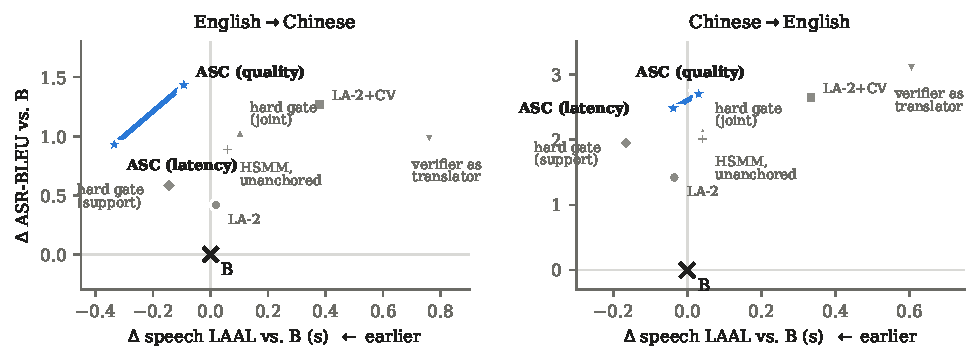
\includegraphics[width=\linewidth]{figures/frontier.pdf}
  \caption{Commit policies on one drafter relative to the local-agreement baseline B (origin), averaged over five test conditions; up-left is better.
  Rule-based combinations of certificates (grey) share one curve; \ours{} (blue; dev-selected quality and latency points) lies above it.}
  \label{fig:frontier}
\end{figure}

We call the resulting method \ours{} (\emph{Anchored Stability Commitment}).
We evaluate it on real interpreting speech~\citep{cheng2024realsi} and on broadcast-style streams under clean, in-distribution and out-of-distribution noise, in both English--Chinese directions.
One bidirectional model is used for every trained component.
\Cref{fig:frontier} summarises the outcome.
At the speech latency of the local-agreement baseline, \ours{} reaches the translation quality of the much slower cross-view system.
Our contributions are:
\begin{itemize}[leftmargin=*,itemsep=1pt,topsep=2pt]
  \item Prefix commitment as filtering of a per-unit settledness state with an input-driven HSMM over certificates whose reliability depends on the acoustics (\cref{sec:hsmm}).
  \item Anchored end-to-end training through the forward algorithm, which ties the latent state to survival and makes a single threshold the Bayes-optimal rule under homogeneous evidence (\cref{sec:anchor,sec:rule}).
  \item A speech-support verifier trained only from aligned references, and boundary healing for subword drafters (\cref{sec:cert,sec:heal}).
  \item An anatomy of the remaining latency showing that the commit layer is near its information limit (\cref{sec:anatomy}).
\end{itemize}

\section{Related Work}
\label{sec:related}

\paragraph{Read/write policies.}
Fixed policies such as wait-$k$~\citep{ma2019stacl} read a constant lead before each write.
Adaptive policies learn when to write through monotonic attention~\citep{arivazhagan2019monotonic,ma2020mma}.
The Hidden Markov Transformer~\citep{zhang2023hmt} treats the moment of each target token as a latent variable.
Other policies use cross-attention for offline speech models~\citep{papi2023attention,papi2023alignatt,papi2024streamatt} or prompt and fine-tune LLMs~\citep{koshkin2024transllama,ouyang2025taf,cheng2025liveinterpret}.
We instead keep a full-sentence speech LLM frozen and decide how much of its revisable draft to commit, as in re-translation with local agreement~\citep{arivazhagan2020retranslation,liu2020low,polak2022cuni,machacek2023turning}.
HMT learns when to write inside the translator; \ours{} infers, from outside a frozen drafter, whether drafted content has settled.

\paragraph{Simultaneous speech-to-speech translation.}
SimulS2ST systems include StreamSpeech~\citep{zhang2024streamspeech}, Seamless~\citep{seamless2023}, Hibiki~\citep{labiausse2025hibiki} and LLM-based systems~\citep{deng2025simuls2s}.
Speech LLMs with an integrated talker~\citep{xu2025qwen3omni,uniss2025} make re-translation attractive, because quality comes from an unmodified offline model.
For speech output, committed text also waits for the talker and earlier audio.
We therefore measure length-adaptive average lagging~\citep{papi2022over} on the playback timeline.

\paragraph{Latent-state models, calibration and stopping.}
HSMMs model explicit durations~\citep{yu2010hsmm}, and input-output HMMs let exogenous inputs drive transitions and emissions~\citep{bengio1995iohmm}; both are classically fitted with EM~\citep{dempster1977em,rabiner1989tutorial}.
Hybrid generative--discriminative objectives combine the two likelihoods~\citep{bishop2007generative}.
We use one to fix the meaning of a latent state whose filtering posterior feeds a decision.
Posterior thresholds solve sequential decisions with linear waiting cost~\citep{wald1948optimum,degroot1970optimal,shiryaev1978optimal}, but only on calibrated posteriors~\citep{guo2017calibration}.
Prompts that end inside a subword token are a known problem.
It is addressed by character- and byte-level marginalisation~\citep{vieira2025characters,phan2025exact} and by token healing~\citep{lundberg2023tokenhealing}.
Commitment in re-translation creates such prompts at every read.

\section{Problem Setting}
\label{sec:setting}

A source utterance arrives as a waveform $\bm{x}$ and is read in chunks of $\Delta$ seconds.
At read $t \in \{1,\dots,T\}$ the system has heard $\bm{x}_{\le t\Delta}$.
The drafter $f$, a speech LLM, returns a draft $\hat{\bm{y}}^{(t)} = (\hat{y}^{(t)}_1,\dots,\hat{y}^{(t)}_{L_t})$, a sequence of $L_t$ translation units (characters for Chinese output, words for English output).
The system keeps a committed length $n_t$ that never decreases.
The committed prefix $\hat{\bm{y}}^{(t)}_{1:n_t}$ is sent to the talker, which turns it into speech that is played as soon as earlier speech has finished.
Every later draft is forced to start with the committed prefix.
At the last read $T$ all remaining units are committed.
We say that position $i$ of draft $t$ \emph{survives} when $\hat{\bm{y}}^{(t)}_{1:i}$ equals the prefix of the final translation $\hat{\bm{y}}^{(T)}_{1:i}$; committing a non-surviving prefix produces speech that the final translation contradicts.

Local agreement with two drafts (LA-2)~\citep{liu2020low,polak2022cuni} sets
$n_t = \max\{n_{t-1}, \operatorname{lcp}(\hat{\bm{y}}^{(t)}, \hat{\bm{y}}^{(t-1)})\}$, where $\operatorname{lcp}$ is the length of the longest common prefix.
With a second acoustic view, the draft $\hat{\bm{y}}'^{(t)}$ of the drafter on a speech-enhanced copy of the audio~\citep{schroeter2023deepfilternet}, the cross-view variant (LA-2+CV) additionally caps the commitment at $\operatorname{lcp}(\hat{\bm{y}}^{(t)}, \hat{\bm{y}}'^{(t)})$.
Both rules are deterministic in agreement events: they cannot weigh evidence by reliability, and each added check can only delay commitment.

\section{Anchored Stability Commitment}
\label{sec:method}

\begin{figure}[t]
\centering
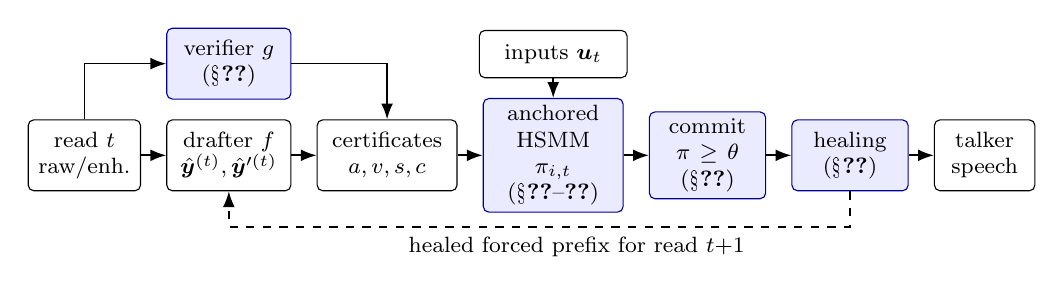
\begin{tikzpicture}[
  font=\footnotesize, >=Latex, node distance=3.2mm,
  box/.style={draw, rounded corners=2pt, align=center, inner sep=2.5pt, minimum height=9mm, text width=14mm},
  ours/.style={box, fill=blue!8, draw=blue!60!black},
  arr/.style={->, semithick}]
\node[box, text width=12.5mm] (x) {read $t$\\raw/enh.};
\node[box, right=of x] (d) {drafter $f$\\$\hat{\bm{y}}^{(t)}, \hat{\bm{y}}'^{(t)}$};
\node[ours, above=2.5mm of d] (g) {verifier $g$\\(\S\ref{sec:cert})};
\node[box, right=of d, text width=16mm] (c) {certificates\\$a, v, s, c$};
\node[ours, right=of c, text width=16mm] (h) {anchored HSMM\\$\pi_{i,t}$ (\S\ref{sec:hsmm}--\ref{sec:anchor})};
\node[box, above=2.5mm of h, text width=17mm, minimum height=6mm] (u) {inputs $\bm{u}_t$};
\node[ours, right=of h, text width=13mm] (r) {commit\\$\pi \ge \theta$ (\S\ref{sec:rule})};
\node[ours, right=of r, text width=13mm] (k) {healing\\(\S\ref{sec:heal})};
\node[box, right=of k, text width=11mm] (t) {talker\\speech};
\draw[arr] (x) -- (d); \draw[arr] (x.north) |- (g.west); \draw[arr] (d) -- (c); \draw[arr] (g.east) -| (c.north);
\draw[arr] (c) -- (h); \draw[arr] (u) -- (h); \draw[arr] (h) -- (r); \draw[arr] (r) -- (k); \draw[arr] (k) -- (t);
\draw[arr, dashed] (k.south) -- ++(0,-4.5mm) -| node[pos=0.22, below]{healed forced prefix for read $t{+}1$} (d.south);
\end{tikzpicture}
\caption{\ours{} at one read. A frozen drafter writes drafts from a raw and an enhanced view; four certificates per position and acoustic inputs are filtered by an HSMM anchored to survival; the longest prefix with $\pi_{i,t} \ge \theta$ is committed. Blue: our components.}
\label{fig:overview}
\end{figure}

\ours{} replaces the agreement rule by three learned parts and one decoding step (\cref{fig:overview}).
The drafter $f$ is never modified, and its draft from the raw view is the only source of committed content.

\subsection{Certificates of Settledness, Including a Speech-Support Verifier}
\label{sec:cert}

A position is committable when its content will not change any more.
No single observable says so, but several observables are correlated with it.
For every uncommitted position $i \in \{n_{t-1}+1,\dots,L_t\}$ of draft $t$ we collect four categorical certificates.
\emph{Temporal agreement} $a_{i,t} \in \{0,1\}$ indicates whether $\hat{\bm{y}}^{(t)}_{1:i} = \hat{\bm{y}}^{(t-1)}_{1:i}$, the event used by LA-2.
\emph{Cross-view agreement} $v_{i,t} \in \{0,1\}$ indicates whether $\hat{\bm{y}}^{(t)}_{1:i} = \hat{\bm{y}}'^{(t)}_{1:i}$.
\emph{Drafter confidence} $c_{i,t} \in \{0,1,2\}$ bins the smallest token probability that $f$ assigned inside unit $i$.
The fourth certificate answers a question that neither drafter view can answer: has the heard speech already expressed the content of position $i$, or is the drafter anticipating it?

Two drafts that complete a sentence alike agree whether or not the speaker has said it.
We therefore train a support verifier $g$, a low-rank adapter~\citep{hu2022lora} on the drafter's backbone that is shared by both translation directions.
Its training data are references with a speech timeline.
For a training pair with reference tokens $(r_1,\dots,r_m)$, a forced aligner and a word aligner give every reference token $r_j$ the earliest read $\rho_j$ at which the source speech supports it (\cref{app:data}).
At read $t$, the supported reference prefix has length $k_t = |\{j : \rho_j \le t\}|$.
The verifier is trained to emit exactly this prefix followed by the end-of-turn token $\langle\mathrm{eot}\rangle$:
\begin{equation}
\mathcal{L}_{g} = -\frac{1}{\sum_t (k_t+1)} \sum_{t=1}^{T} \Big[\sum_{j=1}^{k_t} \log p_g\big(r_j \mid \bm{x}_{\le t\Delta}, \bm{r}_{<j}\big) + \log p_g\big(\langle\mathrm{eot}\rangle \mid \bm{x}_{\le t\Delta}, \bm{r}_{\le k_t}\big)\Big],
\label{eq:sap}
\end{equation}
with the full reference as the target at the final read; no other model's outputs are used.
At inference, $g$ continues the committed prefix greedily on the raw view and stops where support ends.
Its output $\hat{\bm{y}}^{\mathrm{sup}(t)}$ gives $s_{i,t} = 0$ if $i > \operatorname{lcp}(\hat{\bm{y}}^{(t)}, \hat{\bm{y}}^{\mathrm{sup}(t)})$, and otherwise one of three bins of $g$'s smallest token probability in unit $i$.
As a translator $g$ is $0.6$--$0.8$\,s too slow (\cref{tab:main}); as a certificate it supplies what agreement lacks.

\subsection{An Input-Driven Hidden Semi-Markov Model of Settledness}
\label{sec:hsmm}

The four certificates disagree often, and how much each one can be trusted depends on the audio.
When the enhancer removes a lot of energy from the new second, cross-view disagreement is mostly an artefact of enhancement; on clean speech it signals real ambiguity.
We therefore model each position with a latent state and let acoustic inputs modulate both the state dynamics and the emissions.

Position $i$ first appears in draft $t^0_i$.
From then on it is in state $z_{i,t} \in \{\Ust, \Sst\}$, unsettled or settled, and $\Sst$ is absorbing.
The switch time $D_i \in \{0,1,\dots\}$ counts the reads after first appearance before the position settles; $D_i = 0$ means that it is settled at first appearance.
Exogenous inputs $\bm{u}_t \in \mathbb{R}^{5}$ describe read $t$.
They are the reliability $r_t \in [0,1]$, the mean frame-level ratio of enhanced to raw energy in the new chunk; the voiced share $e_t$; the age of the position $t - t^0_i$; the read index $t$; and the translation direction $\ell \in \{0,1\}$.
The duration prior is a discrete hazard model,
\begin{equation}
P(D_i = 0) = \sigma\big(\phi_0(\bm{u}_{t^0_i})\big), \qquad
P(D_i = d) = \big(1 - \sigma(\phi_0(\bm{u}_{t^0_i}))\big) \prod_{k=1}^{d-1}\big(1 - \eta_{i,k}\big)\, \eta_{i,d}, \quad d \ge 1,
\label{eq:hazard}
\end{equation}
where $\eta_{i,k} = \sigma(\phi(\bm{u}_{t^0_i + k}))$ is the probability of settling at the $k$-th read after first appearance, $\sigma$ is the logistic function, and $\phi_0, \phi$ are small multilayer perceptrons.

Given the state, the certificates are emitted independently, with logits that are linear in reliability features $\bm{\psi}_t = [1, r_t, r_t^2, \ell]^\top$:
\begin{equation}
p(v_{i,t} \mid z_{i,t}, \bm{u}_t) = \operatorname{softmax}\big(\mathbf{W}^{v}_{z_{i,t}} \bm{\psi}_t\big)_{v_{i,t}},
\label{eq:emission}
\end{equation}
and likewise for $s_{i,t}$ with $\mathbf{W}^{s}_{z}$.
The drafter confidence $c_{i,t}$ uses $\mathbf{W}^{c}_{z}[1,\ell]^\top$.
Temporal agreement compares two consecutive drafts, so it is emitted by the state at the previous read.
A position that was already settled must agree: $p(a_{i,t} = 1 \mid z_{i,t-1} = \Sst) = 1 - \epsilon$ with a small constant $\epsilon$, while under $\Ust$ the agreement probability is again of the form~\eqref{eq:emission}.
This determinism constraint is what makes $\Sst$ mean ``content fixed'' rather than ``evidence looks good''.
Training sequences of positions that are never committed early end with the agreement observed at the final read, which reveals whether the position survived.

Writing $\bm{o}_{i,t} = (a_{i,t}, v_{i,t}, s_{i,t}, c_{i,t})$, the filtering posterior is an exact sum over switch times,
\begin{equation}
\pi_{i,t} = P\big(z_{i,t} = \Sst \mid \bm{o}_{i,t^0_i:t}, \bm{u}\big)
= \frac{\sum_{d=0}^{t - t^0_i} P(D_i = d)\, \Lambda_{i,t}(d)}{\sum_{d=0}^{t - t^0_i} P(D_i = d)\, \Lambda_{i,t}(d) + P(D_i > t - t^0_i)\, \Lambda_{i,t}(\infty)},
\label{eq:posterior}
\end{equation}
where $\Lambda_{i,t}(d)$ is the likelihood of the observations from $t^0_i$ to $t$ when the switch happens $d$ reads after first appearance: $\Ust$-emissions before the switch and $\Sst$-emissions after it.
Durations are truncated at $D_{\max}$ reads.
The cost per position and read is $O(D_{\max})$, negligible next to a drafter call.
The same model serves both directions; $\ell$ enters only as an input.

\subsection{Anchored End-to-End Training}
\label{sec:anchor}

All parameters $\Theta = \{\phi_0, \phi, \mathbf{W}^{a}, \mathbf{W}^{v}, \mathbf{W}^{s}, \mathbf{W}^{c}\}$ are trained by back-propagation through the forward recursion.
We collect rollouts of the drafter under LA-2+CV on open training audio with simulated noise; this gives a set $\mathcal{I}$ of draft positions, each with its certificate sequence.
The generative part of the objective is the exact marginal log-likelihood $\log p_\Theta(\bm{o}_i \mid \bm{u})$, obtained by summing~\eqref{eq:hazard} against the emissions over all switch times.
Its gradient equals the expected complete-data gradient (Fisher's identity), so maximising it is a gradient form of EM~\citep{dempster1977em} that lives in the same graph as the networks $\phi_0, \phi$.

Maximum likelihood alone fails here.
The model may let the absorbing state explain any cluster of evidence, and it picks the most coherent one, ``verifier-supported and agreed across views''.
Positions that agree across reads but not across views are then explained as $\Ust$, and the posterior becomes pessimistic and miscalibrated (\cref{sec:calib}).
Richer emission structures only redistribute mass; the state itself must be tied to the quantity the decision needs.

We anchor it with the survival labels that the rollouts provide for free.
For every pair $(i,t)$ in which position $i$ is uncommitted at a non-final read $t$, let $\varsigma_{i,t} = 1$ if the prefix $\hat{\bm{y}}^{(t)}_{1:i}$ survives to the final translation and $0$ otherwise.
Committed reads are excluded because committed text survives by construction.
The training objective is
\begin{equation}
\mathcal{L}(\Theta) = -\sum_{i \in \mathcal{I}} \log p_\Theta(\bm{o}_i \mid \bm{u})
\;-\; \beta \sum_{(i,t) \in \mathcal{A}} \Big[\varsigma_{i,t} \log \pi_{i,t} + (1 - \varsigma_{i,t}) \log (1 - \pi_{i,t})\Big],
\label{eq:anchor}
\end{equation}
where $\mathcal{A}$ is the set of labelled pairs and $\pi_{i,t}$ is the filtering posterior~\eqref{eq:posterior}.
This is the exact quantity used online, computed in the same graph by a cumulative log-sum-exp over switch times.
The second term is a hybrid generative--discriminative objective~\citep{bishop2007generative}.
It does not replace the HSMM by a classifier: duration prior, reliability-dependent emissions and the determinism constraint keep their roles.
The term only fixes the meaning of $\Sst$.
The labels come from the policy's own rollouts on training data, not from a teacher model.

\subsection{Commitment as Optimal Stopping}
\label{sec:rule}

With a calibrated settledness posterior, the commit rule can be simple:
\begin{equation}
n_t = n_{t-1} + \max\big\{k \ge 0 : \pi_{n_{t-1}+j,\,t} \ge \theta \ \text{ for all } 1 \le j \le k\big\},
\label{eq:rule}
\end{equation}
that is, the longest uncommitted run whose posterior clears a threshold $\theta$; temporal and cross-view agreement enter only as evidence and no longer as hard caps.
We rely on a single threshold because, for a well-calibrated posterior, richer rules have little room to help.
The following proposition makes this precise.

\begin{proposition}[Threshold optimality under homogeneous evidence]
\label{prop:threshold}
Consider one unit whose survival $Y \in \{0,1\}$ is unknown.
At each read the committer either commits, paying $\kappa > 0$ if $Y = 0$, or waits, paying $\lambda > 0$ and receiving new evidence.
Assume the evidence is conditionally i.i.d.\ given $Y$, that a non-surviving unit may be revealed by revision at a constant rate, and that the horizon is unbounded.
Then a constant $\theta^\star \in [0,1]$ exists such that committing at the first read with $P(Y = 1 \mid \text{evidence}) \ge \theta^\star$ is Bayes-optimal.
\end{proposition}

The proof (\cref{app:proof}) shows that the continuation value is concave in the posterior while the commit cost $\kappa(1-\pi)$ is linear and vanishes at $\pi = 1$, so the stopping region is an interval $[\theta^\star, 1]$, a one-sided analogue of the optimality of the sequential probability ratio test~\citep{wald1948optimum}.
The proposition explains why anchoring matters, since the threshold is optimal only on a calibrated survival posterior, and why queue-aware, blocking-aware and regret-based rules hardly improve on~\eqref{eq:rule} (\cref{sec:anatomy}).
$\theta$ is selected once on a development set and sets the operating point.

\subsection{Boundary Healing for Subword Drafters}
\label{sec:heal}

Commitment operates on characters and words, whereas the drafter writes subword tokens.
When $n_t$ ends inside a token, for instance after the first character of a two-character Chinese token, the next draft must continue from a token split the drafter never saw in training, and its continuations are markedly worse.
Boundary healing~\citep{lundberg2023tokenhealing} keeps the commitment but repairs the next prompt.
Let $b \le n_t$ be the character offset of the last token boundary of the draft that precedes the commitment end.
The next read forces only the prefix up to $b$ into the prompts of the drafter, both views, and of the verifier.
Decoding is then constrained by structured decoding so that the first generated characters reproduce the rolled-back span between $b$ and the commitment end, and those characters are stripped from the output.
The drafter continues from its canonical tokenization, the committed speech is unchanged, and commit times are unaffected; character-level marginalisation~\citep{vieira2025characters,phan2025exact} would be an exact alternative.

\section{Experiments}
\label{sec:exp}

\subsection{Setup}
\label{sec:setup}

\paragraph{System.}
The drafter is a Qwen3-Omni thinker~\citep{xu2025qwen3omni} fine-tuned for S2ST~\citep{uniss2025}, with a noise-robust encoder adapter merged by weight interpolation~\citep{wortsman2022robust}.
Reads are $\Delta = 1$\,s apart, and DeepFilterNet3~\citep{schroeter2023deepfilternet} produces the enhanced view.
The UniSS talker speaks the committed text with a voice prompt chosen by analysis-by-synthesis (\cref{app:voice}), and a playback simulator plays it without extra buffering.
Drafter, verifier and HSMM are each one model for both directions; hyperparameters are in \cref{app:hparams}.

\paragraph{Data.}
Training uses open data only: 20{,}000 noisy UniST~\citep{uniss2025} pairs per direction for the verifier, and LA-2+CV rollouts on 3{,}000 further noisy sentences per direction for the HSMM.
$\theta$ is selected on held-out spontaneous UniST sentences, clean and noisy.
The test benchmark has five conditions per direction.
RealSI~\citep{cheng2024realsi} provides real interpreting-style speech from ten domains, both clean and mixed with held-out noise.
OpenBroadcast-SI (OBSI) is built from CoVoST~2 test speech~\citep{wang2020covost2}, concatenated into multi-speaker broadcast-style streams.
It comes in three conditions: clean; \emph{id} noise, which uses held-out clips of the background types seen in training; and \emph{ood} noise, which uses background corpora never used in training.
The test sets were used only for final evaluation.
\Cref{app:data} gives sizes and construction.

\paragraph{Metrics.}
Quality is ASR-BLEU, using Whisper-large-v3~\citep{radford2023robust} for English and Paraformer~\citep{gao2023funasr} for Chinese, with sacreBLEU~\citep{post2018call}; we also report text BLEU.
The primary latency metric is speech LAAL~\citep{papi2022over}, computed from each unit's playback start on the computed playback timeline.
We also report EndOffset (source end to output end) and within-utterance pauses (NP).
Speaker similarity (ECAPA2~\citep{thienpondt2023ecapa2}) and PESQ (SQUIM~\citep{kumar2023squim}) are in \cref{app:full}.
Numbers are means over the five conditions of a direction, with paired bootstrap intervals~\citep{koehn2004statistical}.

\paragraph{Baselines.}
\textbf{B} uses the backbone without the robust adapter, LA-2 and the source voice.
All other systems share drafter, talker, voice and playback, and differ only in the commit policy.
\textbf{LA-2} and \textbf{LA-2+CV} (\cref{sec:setting}); LA-2+CV was the strongest prior configuration of this drafter.
\textbf{Verifier as translator} speaks $g$'s own draft.
\textbf{Hard gates} commit beyond LA-2 where the verifier supports the text, capped by cross-view agreement, or where drafter and verifier are both confident.
\textbf{HSMM, unanchored} is trained by maximum likelihood alone, with its best dev rule.

\subsection{Main Results}
\label{sec:main}

\begin{table}[t]
\centering
\caption{Test results, mean of five conditions per direction; LAAL is speech LAAL (s).
Rows below B differ only in the commit policy.
\ours{} rows include healing and a faster talker rate ($\le$0.02\,s LAAL effect, \cref{tab:abl}).}
\label{tab:main}
\small
\setlength{\tabcolsep}{4.5pt}
\begin{tabular}{lcccccc}
\toprule
& \multicolumn{3}{c}{\enzh{}} & \multicolumn{3}{c}{\zhen{}} \\
\cmidrule(lr){2-4}\cmidrule(lr){5-7}
Commit policy & ASR-BLEU$\uparrow$ & BLEU$\uparrow$ & LAAL$\downarrow$ & ASR-BLEU$\uparrow$ & BLEU$\uparrow$ & LAAL$\downarrow$ \\
\midrule
\tabinput{generated/tab_main.tex}
\bottomrule
\end{tabular}
\end{table}

\paragraph{Does filtering beat combining certificates by rules?}
\Cref{tab:main} and \cref{fig:frontier} show that it does.
Every hard combination of the same certificates lands on one curve.
The cross-view constraint buys quality with latency, while a support-gated rule buys latency with quality.
The unanchored HSMM falls on the same curve.
\ours{} at $\theta = 0.75$ sits above it.
In both directions it reaches the ASR-BLEU of LA-2+CV, while its speech LAAL is 0.47\,s (\enzh{}) and 0.30\,s (\zhen{}) lower, close to that of B.
Against LA-2 on the same drafter it gains 1.02 and 1.28 ASR-BLEU at $-0.11$ and $+0.07$\,s; against B, 1.43 and 2.70 at $-0.09$ and $+0.03$\,s.
This confirms the premise of \cref{sec:hsmm}: weighing certificates by their reliability lets the commit layer keep the quality of the conservative rule without paying its delay.

\paragraph{Is the gain an operating point or a better curve?}
The dev-selected latency point is 0.34\,s (\enzh{}, $\theta = 0.60$) and 0.04\,s (\zhen{}, blocking-aware threshold, \cref{app:blocking}) earlier than B, and still 0.93 and 2.48 ASR-BLEU better.
Every other system is dominated by one of the two \ours{} points, except the slow verifier-as-translator and the \zhen{} support gate, which is 0.13\,s earlier but 0.53 ASR-BLEU lower (\cref{fig:frontier}).
The curve itself has shifted.

\begin{table}[t]
\centering
\caption{Per-condition differences to B: $\Delta$ASR-BLEU / $\Delta$speech LAAL (s).
Bold marks a 95\% paired bootstrap interval that excludes zero.
Absolute B values are in \cref{app:full}.}
\label{tab:cells}
\small
\setlength{\tabcolsep}{3.2pt}
\resizebox{\linewidth}{!}{%
\begin{tabular}{llccccc}
\toprule
& & \multicolumn{2}{c}{RealSI} & \multicolumn{3}{c}{OBSI} \\
\cmidrule(lr){3-4}\cmidrule(lr){5-7}
System & Dir. & clean & noisy & clean & id noise & ood noise \\
\midrule
\tabinput{generated/tab_cells.tex}
\bottomrule
\end{tabular}}
\end{table}

\paragraph{Where does it help?}
ASR-BLEU improves in all 20 system--condition pairs of \cref{tab:cells}, most in noisy conditions (up to $+4.5$).
The latency point is earlier than B in every \enzh{} condition, including real interpreting speech, and in four of five \zhen{} conditions.
Noisy RealSI \zhen{}, fast spontaneous speech in real noise, remains the hardest case: the posterior stays cautious and trades $+4.3$ to $+4.5$ ASR-BLEU for 0.14--0.24\,s.

\subsection{Anchoring Makes the Posterior Usable}
\label{sec:calib}

\begin{table}[t]
\centering
\caption{Posterior calibration on held-out training rollouts (54{,}285 uncommitted position--reads; survival 0.48). Right: survival of positions with $\pi_{i,t} < 0.1$ after $k$ observed reads.}
\label{tab:calib}
\small
\setlength{\tabcolsep}{4pt}
\begin{tabular}{lccccccc}
\toprule
& & & & \multicolumn{4}{c}{Low-$\pi$ survival after $k$ reads} \\
\cmidrule(lr){5-8}
HSMM training & ECE$\downarrow$ & AUC$\uparrow$ & mean $\pi$ & $k{=}1$ & $k{=}2$ & $k{=}3$ & $k{\ge}4$ \\
\midrule
Maximum likelihood & 0.310 & 0.727 & 0.18 & 0.31 & 0.40 & 0.47 & 0.51 \\
Anchored (\cref{eq:anchor}) & \textbf{0.084} & \textbf{0.744} & 0.42 & 0.16 & 0.23 & 0.32 & 0.38 \\
\bottomrule
\end{tabular}
\end{table}

\paragraph{Does maximum likelihood learn the state the decision needs?}
It does not (\cref{tab:calib}).
The unanchored posterior averages 0.18 while 48\% of positions survive.
Positions below 0.1 survive 31--51\% of the time, more so the longer they have been observed, because each read repeats correlated evidence.
Survival is also flat (0.71--0.74) for posteriors between 0.3 and 0.7, so no threshold works, and the unanchored HSMM must fall back to the agreement rule.
Correlation-aware emissions lowered ECE only to 0.21 and lost AUC (\cref{app:negative}).
Anchoring cuts ECE to 0.084, raises AUC, and moves positions that agree across reads but not across views from $\pi \approx 0.02$ to $\pi \approx 0.7$.
Only then does the pure threshold~\eqref{eq:rule} become the best rule on dev, as \cref{prop:threshold} predicts.

\subsection{Boundary Healing}
\label{sec:healres}

\paragraph{Do sub-token commitments hurt?}
They do, in \enzh{}, where 8.6\% of non-final commitments end inside a multi-character token.
On dev, healing raises BLEU from 58.62 to 59.26 at unchanged proxy latency (2.817 vs.\ 2.801\,s); snapping commitments back to the boundary gives the same BLEU but delays speech, because it withholds ready characters.
On test, healing adds 0.56 ASR-BLEU in \enzh{} (\cref{tab:abl}); its decoding constraint never failed in 525 uses.
English word units never end inside a token, so the \zhen{} differences are run-to-run noise (about 0.1--0.15 ASR-BLEU).
Any re-translation system with a subword drafter must reconcile commit units with tokens, or the commit rule silently damages the drafts it relies on.

\subsection{Anatomy of the Remaining Latency}
\label{sec:anatomy}

\paragraph{How close is the commit layer to its limit?}
A unit is written correctly and stable within 0.15\,s, but about half of the units then wait one more read before commitment (\cref{tab:anatomy}, \cref{app:anatomy}); this read is the controllable latency.
Extra certificates, denser reads, queue-aware thresholds and regret-based commitment all failed to save it.
Half-second reads cut speech LAAL by almost a second but cost 9--10 BLEU: the next second of audio really decides whether a guess is right.
Within the drafter's anticipations the posterior reaches AUC $\approx 0.8$, and no further certificate added more than 0.02.
With \cref{prop:threshold}, a calibrated threshold is thus close to the best a commit layer can do with a frozen drafter.
Further gains must come from the drafter, and the information exists: given the true source text so far, the frozen drafter ranks the next second's first source token in its top five 58.6\% (English) and 38.2\% (Chinese) of the time, against 17.3\% and 6.3\% for a frequency prior.

\subsection{Ablation Analysis}
\label{sec:abl}

\begin{table}[t]
\centering
\caption{Test ablations: differences to B, mean of five conditions (ASR: ASR-BLEU; LAAL: speech, s; EO: EndOffset, s; NP: pauses per utterance).}
\label{tab:abl}
\small
\setlength{\tabcolsep}{3pt}
\begin{tabular}{lcccccccc}
\toprule
& \multicolumn{4}{c}{\enzh{}} & \multicolumn{4}{c}{\zhen{}} \\
\cmidrule(lr){2-5}\cmidrule(lr){6-9}
Variant & ASR & LAAL & EO & NP & ASR & LAAL & EO & NP \\
\midrule
\tabinput{generated/tab_abl.tex}
\bottomrule
\end{tabular}
\end{table}

\Cref{tab:abl} removes components one at a time.
\textbf{Anchoring} matters most: against the matching configuration (no healing, default rate), the unanchored HSMM is 0.12\,s later at equal ASR-BLEU in \enzh{} and 0.43 ASR-BLEU lower at equal latency in \zhen{}.
\textbf{Healing} adds 0.56 ASR-BLEU in \enzh{} at no latency cost.
\textbf{The talker rate}, a playback-layer setting reported only for fair comparison, shortens EndOffset by 0.14--0.29\,s and moves speech LAAL by at most 0.02\,s.
\textbf{The threshold} trades as expected: $\theta = 0.80$ is 0.10--0.13\,s later than $0.75$ for $+0.08$ and $+0.38$ ASR-BLEU.
Two extensions did not help: a distance-to-draft-end input raised held-out AUC from 0.744 to 0.766 yet made the test system slower and worse, and refitting on the policy's own rollouts made \zhen{} slower.
The commit layer lacks information, not capacity (\cref{sec:anatomy}).
Pauses are the price of earlier commitment: the certificate-based policies add 0.15--0.31 within-utterance pauses per utterance relative to B, because shorter commitments leave the playback queue empty more often.

\section{Conclusion}
\label{sec:conclusion}

We recast prefix commitment in re-translation as filtering of a latent settledness state from unreliable certificates, with an input-driven HSMM whose training is anchored to survival so that a single threshold is the right rule.
With a support verifier and boundary healing, \ours{} reaches the quality of a conservative cross-view system at the latency of local agreement, using one bidirectional model.
The remaining avoidable latency is one informative read after a unit settles; drafters that carry more predictive information about upcoming speech~\citep{gloeckle2024better} are the natural next step.

\paragraph{Limitations.}
One language pair, one drafter family and 1\,s reads; earlier commitment adds pauses; latency is computed on a simulated playback timeline without a listening test.

\paragraph{Ethics statement.}
Simultaneous translation that clones the speaker's voice can be misused for impersonation.
Our voice pipeline only conditions on the current speaker's own speech.
All training data are openly licensed corpora, and the test sets are used for evaluation only.

\paragraph{Reproducibility statement.}
\Cref{app:hparams} lists all hyperparameters, \cref{app:data} the data construction, and \cref{app:proof} the proof of \cref{prop:threshold}.
Every design change was registered in a dated log before its results were computed (\cref{app:negative}).
We will release code, the trained verifier and HSMM, and the benchmark construction scripts.


\bibliography{references}
\bibliographystyle{iclr2026_conference}

\appendix
\section{Training Implementation Details and Hyperparameters}
\label{app:hparams}

\paragraph{Drafter and decoding.}
The drafter is the thinker of Qwen3-Omni-30B-A3B fine-tuned for zh$\leftrightarrow$en S2ST~\citep{uniss2025}.
A noise-robust low-rank adapter on its audio encoder, trained on noisy UniST audio, is merged with interpolation weight 0.5~\citep{wortsman2022robust}.
The drafter is frozen in all experiments of this paper.
Drafts are decoded greedily with vLLM; the raw-view prompt and the enhanced-view prompt are batched at the same read.
Units are Chinese characters for Chinese output and whitespace-delimited words for English output.
Reads are $\Delta = 1$\,s apart; the last read covers the remainder of the utterance.

\paragraph{Support verifier.}
Low-rank adapter with rank 16 and scaling 32 on the query, key, value and output projections of all 48 text layers; audio encoder frozen.
AdamW, learning rate $10^{-4}$, 50 warm-up steps, cosine decay, 1{,}000 steps of 16 sentences on 8 GPUs (about 56 minutes on H200), seed 20261125.
All reads of a sentence are teacher-forced in one batch.
The waiting token of the backbone is masked out.
At inference, the adapter is served as a LoRA request on the same engine as the drafter.
Confidence bins for $s_{i,t}$ and $c_{i,t}$ use the smallest token probability in the unit, with thresholds 0.9 and 0.5.

\paragraph{HSMM.}
$\phi_0$ and $\phi$ are multilayer perceptrons $5 \rightarrow 16 \rightarrow 1$ with $\tanh$ activations.
Inputs are $[r_t, e_t, (t - t^0_i)/10, t/10, \ell]$.
$r_t$ is the mean over 20\,ms frames of the new second of the energy ratio between enhanced and raw audio, clipped to $[0,1]$; near-silent frames count as 1, so $r_t$ is low when the enhancer removes much energy.
$e_t$ is the share of raw frames above $-40$\,dBFS.
Emission features are $[1, r_t, r_t^2, \ell]$, and $[1, \ell]$ for drafter confidence.
Further constants: $D_{\max} = 16$ reads, $\epsilon = 10^{-3}$, $\beta = 1$.
Emissions are initialised uniformly.
Training uses Adam with learning rate $10^{-2}$, mini-batches of 4{,}096 position sequences, 60 epochs and seed 20261125.
Rollouts come from LA-2+CV on 3{,}000 noisy UniST sentences per direction, merged across directions into one training set.
The training-time filtering posterior agrees with the online implementation to $4 \times 10^{-7}$.
Fitting runs on CPU in minutes.

\paragraph{Operating points.}
$\theta$ is selected on the development set with a fixed rule.
Among configurations whose BLEU is within 0.30 of a reference configuration, we take the one with the lowest proxy speech delay.
The quality point uses $\theta = 0.75$ in both directions.
The latency point uses $\theta = 0.60$ for \enzh{} and $\theta = 0.75$ with the blocking-aware rule ($\kappa = 0.10$, \cref{app:blocking}) for \zhen{}.

\paragraph{Boundary healing.}
Token boundaries are the character offsets at which the drafter's tokenizer splits the current draft.
The rolled-back span is enforced through vLLM structured decoding (a pattern that must start with the span) and is removed from the output.

\paragraph{Talker rate.}
The talker accepts a discrete speaking-rate token.
\ours{} rows raise it by one step globally and by three steps for the block written after the source has ended.
All other systems use the default rate policy.

\section{Data and Benchmarks}
\label{app:data}

\paragraph{Training data.}
UniST zh$\leftrightarrow$en rows~\citep{uniss2025} whose source and target speech pass automatic transcription checks, with source durations of 3--15\,s.
Rows whose source or target text overlaps any evaluation or test source are removed.
We take 20{,}000 rows per direction for the verifier and a disjoint held-out pool for development.
Each training sample stays clean with probability 0.5; otherwise one background type (music, crowd or sound effects) is mixed in.
The background-to-voice ratio is sampled from quantiles of an open development benchmark, never from test data.

\paragraph{Support times.}
Source and target words are time-aligned with a forced aligner, and target words are linked to source words by a word aligner.
The support time of a target word is the earliest prefix after which the backbone's log-probability of the word stays within $\log 2$ of its final value.
It is never earlier than the moment its high-confidence source links have been heard.
A reference token is supported at read $\rho_j = \lceil \text{support time} / \Delta \rceil$, made monotone by a running maximum.

\paragraph{Development set.}
646 \enzh{} and 1{,}000 \zhen{} held-out spontaneous UniST sentences, each in a clean and a noisy version: 1{,}292 and 2{,}000 items.

\paragraph{Test sets.}
RealSI~\citep{cheng2024realsi}: 346 \enzh{} and 431 \zhen{} sentences, clean and mixed with held-out backgrounds.
One \enzh{} clean sentence on which the drafter degenerates into repetition is removed for all systems.
OpenBroadcast-SI (OBSI): CoVoST~2 test speech~\citep{wang2020covost2}, concatenated into streams of 2--4 speakers and scored on 585 (\enzh{}) and 678 (\zhen{}) windows per condition.
The \emph{id-noise} condition mixes held-out clips of MUSAN-style music and noise and FSD50K events, background types seen in training.
The \emph{ood-noise} condition uses instrumental FMA-small music, DEMAND crowded environments and ESC-50 sound effects, corpora never used in training.
All three OBSI conditions share the same speech.

\section{Proof of Proposition~\ref{prop:threshold}}
\label{app:proof}

Let $\pi \in [0,1]$ be the posterior probability that $Y = 1$.
Because the evidence is conditionally i.i.d.\ given $Y$ and revision of a non-surviving unit occurs at a constant rate, $\pi$ is a sufficient statistic.
Its one-step transition does not depend on time.
Committing costs $C(\pi) = \kappa(1 - \pi)$.
Waiting costs $\lambda$, followed by either a revision, which ends the problem at no further cost, or a new posterior $\pi'$.

Fix any policy $\sigma$, that is, a map from observation histories to actions.
Conditioned on $Y$, its expected total cost $J_\sigma(Y)$ does not depend on the prior.
Hence its expected cost under prior $\pi$, $J_\sigma(\pi) = \pi J_\sigma(1) + (1-\pi) J_\sigma(0)$, is affine in $\pi$.
The optimal value $V(\pi) = \inf_\sigma J_\sigma(\pi)$ is an infimum of affine functions and therefore concave.
The same argument applies to the continuation value $W(\pi)$, the infimum over policies that wait at the first step.
By the Bellman equation $V(\pi) = \min\{C(\pi), W(\pi)\}$, it is optimal to commit exactly on the set $\mathcal{S} = \{\pi : C(\pi) \le W(\pi)\}$.
The function $W - C$ is concave, being concave minus affine.
Moreover $W(1) \ge \lambda > 0 = C(1)$.
The super-level set $\{\pi : W(\pi) - C(\pi) \ge 0\}$ of a concave function is an interval, and this one contains $1$, so $\mathcal{S} = [\theta^\star, 1]$ for some $\theta^\star$.
Since $W$ does not depend on time under stationarity and an unbounded horizon, $\theta^\star$ is constant.
The optimal policy commits at the first read with $\pi \ge \theta^\star$.
This is the one-sided version of the classical Bayes solution to sequential testing~\citep{wald1948optimum,degroot1970optimal,shiryaev1978optimal}. \hfill$\square$

When evidence quality changes over time, or the horizon is finite, $W$ depends on time and the optimal threshold may drift.
The HSMM absorbs part of this non-stationarity through the age and time inputs of its hazard and the reliability inputs of its emissions.
Coupling between units, for example through the shared playback queue or blocked positions, also violates the assumptions.
\Cref{app:blocking} and \cref{tab:anatomy} test such couplings.

\section{Voice and Talker Pipeline}
\label{app:voice}

All systems except B condition the talker on a voice prompt chosen at the first write.
A speaker-embedding posterior is computed by a closed-form isotropic Kalman update~\citep{kalman1960new} over per-second TitaNet embeddings~\citep{koluguri2022titanet}.
Each segment embedding is projected by a learned linear residual map and weighted by a learned, reliability-dependent precision.
This filter was trained end to end in earlier work of ours on open LibriSpeech and AISHELL-1 mixtures.
Its posterior mean at the first write is the target of an analysis-by-synthesis search over the talker's global voice tokens~\citep{wang2025spark}.
The search scores re-synthesised candidates by cosine similarity to the target.
The same model also contains a learned onset gate; we do not use it, because it learned never to wait.
Compared with a target computed from the whole prompt, the Kalman target gives equal or slightly lower speaker similarity (by at most 0.01).
The similarity and PESQ gains over B in \cref{app:full} come mainly from the search, which is identical for all non-B rows.
B uses the source speech as the voice prompt.

\section{Blocking-Aware Threshold}
\label{app:blocking}

Waiting on an uncertain position also delays every position behind it.
Let $j$ be the first position after the threshold cut~\eqref{eq:rule}.
Let $b_j$ be the number of consecutive positions after $j$ whose posterior clears $\theta$.
The blocking-aware rule additionally commits $j$ together with these $b_j$ positions, and then continues, if
$\pi_{j,t} \ge \max\{0.5,\ 1 - \kappa(1 + b_j)\}$.
This is a simplification of Weitzman's reservation-value rule~\citep{weitzman1979optimal} for the case where the next read resolves a position with constant probability.
The single scalar $\kappa$ prices the delay of each blocked position.
On the development set it reduces \zhen{} proxy latency by 0.061\,s at $-0.18$ BLEU.
In \enzh{} it is no better than lowering $\theta$.
In \zhen{}, a plain lower threshold reaches the same development BLEU only 0.02\,s later (from separate runs), so in both directions the rule acts as a lower threshold.

\section{Full Results}
\label{app:full}

\begin{table}[h]
\centering
\caption{All metrics on the test set, averaged over five conditions; differences to B (first row of each block: absolute B values).
LAAL$_s$/LAAL$_t$: speech/text LAAL (s); EO: EndOffset (s); NP/PT: within-utterance pauses per utterance and their total duration (s); Sim: ECAPA2 speaker similarity; PESQ: SQUIM estimate.
Sim and PESQ differences are medians of paired differences.}
\label{tab:full}
\scriptsize
\setlength{\tabcolsep}{2.6pt}
\begin{tabular}{lccccccccc}
\toprule
System & ASR-BLEU & BLEU & LAAL$_s$ & LAAL$_t$ & EO & NP & PT & Sim & PESQ \\
\midrule
\tabinput{generated/tab_full.tex}
\bottomrule
\end{tabular}
\end{table}

\begin{table}[h]
\centering
\caption{Absolute ASR-BLEU / speech LAAL (s) of B per condition.}
\label{tab:babs}
\small
\setlength{\tabcolsep}{3.2pt}
\begin{tabular}{llccccc}
\toprule
& & \multicolumn{2}{c}{RealSI} & \multicolumn{3}{c}{OBSI} \\
\cmidrule(lr){3-4}\cmidrule(lr){5-7}
System & Dir. & clean & noisy & clean & id noise & ood noise \\
\midrule
\tabinput{generated/tab_cells_b.tex}
\bottomrule
\end{tabular}
\end{table}

\section{Latency Anatomy}
\label{app:anatomy}

\begin{table}[h]
\centering
\caption{Where latency remains and why richer commit rules do not remove it (development set; \enzh{} / \zhen{} where two values are given).}
\label{tab:anatomy}
\small
\setlength{\tabcolsep}{4pt}
\begin{tabular}{p{0.30\linewidth}p{0.62\linewidth}}
\toprule
\multicolumn{2}{l}{\textit{Timeline of a unit under \ours{} (without healing)}} \\
first correct $\rightarrow$ settled & 0.07--0.15\,s \\
settled $\rightarrow$ committed & same read 44\% / 49\%; one read later 48\% / 42\%; $\ge$2 reads 8\% / 9\%; mean 0.56 / 0.52\,s \\
committed only at the final read & 36\% / 38\% of units \\
\midrule
\multicolumn{2}{l}{\textit{Attempts to save the extra read}} \\
more certificates & distance to draft end, sampled-continuation consistency ($K{=}6$), correlation-aware emissions: held-out AUC changes from $-0.010$ to $+0.022$; no test gain \\
denser reads (0.5\,s) & speech LAAL $-0.95$\,s but BLEU $-9$ to $-10$: the next second of audio is genuinely informative \\
queue-aware threshold & commits only when the playback queue would otherwise idle: fewer pauses, speech LAAL $+0.13$ to $+0.22$\,s \\
regret-based commit & early commits are costly when wrong (sentence BLEU $-6$ to $-8$ for non-surviving units); harm is predictable only at AUC 0.69--0.74 \\
lower $\theta$ & moves along the curve at roughly 0.3--0.5\,s per BLEU point \\
\bottomrule
\end{tabular}
\end{table}

\section{Development Log and Negative Results}
\label{app:negative}

Every change was registered in a dated log before its numbers were computed.
The test sets were scored only for registered configurations.
The following designs were registered, run, and did not improve the system:
\begin{itemize}[leftmargin=*,itemsep=1pt]
  \item \textbf{Unsupervised HSMMs with per-direction parameters} were replaced by one joint model, to satisfy the single-model constraint; neither was calibrated without anchoring.
  \item \textbf{Correlation-aware emissions}: a joint categorical over the certificate tuple, conditioned on the previous read's evidence. ECE fell from 0.310 to 0.208, but AUC dropped by 0.010.
  \item \textbf{A risk-budget prefix rule} allowed commitment across a single low-posterior dip. Development BLEU fell by 2.6--3.9: the dips are real revision points.
  \item \textbf{Queue-aware commitment} commits only when the playback queue would otherwise idle. It gives fewer pauses but 0.13--0.22\,s more speech LAAL.
  \item \textbf{Sampled-continuation consistency} ($K = 6$ samples per read) runs in real time, with per-read 95th-percentile overhead of 236--286\,ms. AUC on anticipated units rose by only 0.010--0.015.
  \item \textbf{Regret-based commitment and half-second reads}: see \cref{tab:anatomy}.
  \item \textbf{Training the drafter to stop at the support boundary}, i.e.\ using the verifier as translator, is 0.6--0.8\,s slower (\cref{tab:main}).
  \item \textbf{Token-level reinforcement learning} with counterfactual branching, and \textbf{evolution strategies}, were tried for the drafter. Pre-checks showed that the pipeline is chaotic under floating-point perturbation: null branches differ in 1.6--2.5\% of units, which swamps the learning signal.
  \item \textbf{Character-exact evidence}: marginalising the drafter's first-token probability over tokens compatible with a healed prefix changed neither BLEU nor latency.
  \item \textbf{A source-future adapter on the drafter}: a LoRA trained to translate full utterances and, at a random read, to transcribe the heard audio and continue with the next second of source speech; the HSMM was refitted on its rollouts.
  At a fixed threshold it commits 0.31\,s earlier on development data and 0.34\,s earlier on test data, so source anticipation does let content settle sooner.
  Its development BLEU rose by 0.9--3.7 points, but \enzh{} test ASR-BLEU fell by 2.5 points at the same threshold, and the loss is concentrated on the broadcast streams (text BLEU $-1.9$ to $-2.3$) rather than on real interpreting ($-0.4$ to $+0.5$).
  The translation term was supervised by training references in the development set's style, which most likely pulled the drafter's wording away from the test references.
\end{itemize}


\end{document}
